\documentclass[12pt]{article}
\usepackage{geometry}
\geometry{a4paper, margin=1in}
\usepackage[utf8x]{inputenc}
\usepackage{listings}
\usepackage{authblk}
\usepackage{graphicx}
\usepackage{amsfonts}
\usepackage{enumitem}
\usepackage{caption}
\usepackage{amssymb}
\usepackage{hyperref}
\usepackage{setspace} % for line spacing adjustment
\usepackage{float} % for H option
% \usepackage{fontspec}
\usepackage{pdfpages}
\usepackage{pdflscape}
\usepackage{placeins}
\usepackage{varwidth}


% Configuration des couleurs des liens
\hypersetup{
    hidelinks,
    colorlinks=true,       % Mettre à true si vous voulez des liens colorés
    linkcolor=lightblue,       % Couleur des liens internes (table des matières, etc.)
    filecolor=black,       % Couleur des liens vers des fichiers locaux
    urlcolor=black,        % Couleur des hyperliens
    citecolor=black  % Couleur des liens vers les références bibliographiques
    pdfborder={0 0 1}
}

% \setmainfont{Lato}
\title{\textbf{Projet Robotique} 

Projet de développement\\
LU2IN013 }
\author{\\Inès BENAMER BELKACEM 21204927\\Claude CHIBOUT 21202978 \\ Maëlle LIU 21204734\\ Thibaut MARCQ 21202966\\ Jérôme YU 21114103}
\date{Semestre 4 - L2}

\begin{document}
\maketitle
\vspace{2cm}
\begin{figure}[h]
  \centering
  \begin{minipage}[t]{0.35\textwidth}
    \centering
    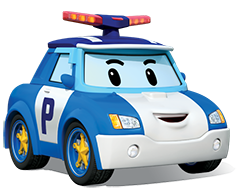
\includegraphics[width=0.8\linewidth]{robocar.png}
    \caption*{Groupe \\ Robocar Poli}
  \end{minipage}
  \hspace{0.05\textwidth} % Espace horizontal entre les images
  \begin{minipage}[t]{0.45\textwidth}
    \centering
    
\includegraphics[width=0.8\linewidth]{Sciences_SU.png}
  \end{minipage}
\end{figure}


\newpage

\renewcommand*\contentsname{Sommaire}
\tableofcontents
\vspace{2cm}
\section*{Liens}
\begin{center}
  \parbox[p]{0.30\textwidth}{
    \subsubsection*{\href{https://github.com/thibautmarcq/projet-2IN013}{Lien Github}}
  }
  \hfill
  \parbox[p]{0.30\textwidth}{
    \subsubsection*{\href{https://trello.com/b/sourGsMk/projet-robocar-poli}{Lien Trello}}
  }
    \hfill
  \parbox[p]{0.30\textwidth}{
    \subsubsection*{\href{https://www.canva.com/design/DAGG5gl8c54/ctSZ7vz2iyxrhtkZ1uaysg/edit?utm_content=DAGG5gl8c54&utm_campaign=designshare&utm_medium=link2&utm_source=sharebuttonhttps://www.canva.com/design/DAGG5gl8c54/ctSZ7vz2iyxrhtkZ1uaysg/edit?utm_content=DAGG5gl8c54&utm_campaign=designshare&utm_medium=link2&utm_source=sharebutton}{Lien Canva (slides)}}
  }
\end{center}

% ---------------------------------------------------------

\newpage
\section*{Objectifs et description du projet}
\addcontentsline{toc}{section}{Objectifs et description du projet}
\\

\hspace{\parindent}Ce projet avait pour but le contrôle d’un robot \textbf{Gopigo} mis à notre disposition, équipé d’un Raspberry Pi et d’une carte Arduino. Nous devions implémenter certaines \textbf{stratégies} autour du mouvement, de la \textbf{gestion de distances}, ainsi que de la \textbf{reconnaissance d’image}. Les stratégies principales étaient : \textbf{tracer un carré} avec le robot, \textbf{avancer jusqu’à un mur} sans se crasher (s’arrêter avant) et \textbf{suivre une balise}.
\\ \\
\hspace{\parindent}Le projet s’est déroulé en deux grandes parties.

%-------------------------------------------------------------------

\subsection*{- Démarrage et Interface 2D}
\addcontentsline{toc}{subsection}{Démarrage et Interface 2D}

\hspace{\parindent}Dans un premier temps, nous avons dû simuler un robot dans un environnement à \textbf{deux dimensions}. Cette partie nous a permis de comprendre, d'un point de vue \textbf{conceptionnel}, le fonctionnement et les interactions du robot avec son environnement, ainsi que l'implémentation de ses fonctions. Nous devions donc simuler : le robot, l’environnement dans lequel il évoluait et les potentiels \textbf{obstacles} qu’il allait rencontrer, le tout dans une \textbf{interface 2D}.

\hspace{\parindent}Nous avons commencé par créer les modules du robot, de l'environnement, du contrôleur et des stratégies. Les trois nous ont permis de former une simulation, représentée par l'interface 2D.

\hspace{\parindent}Nous avons choisi d'utiliser \textbf{Tkinter} pour cette interface. C’est un module Python très facile à utiliser de part la simplicité de ses fonctions, et du fait qu’il soit directement intégré à Python. Nous l'avons préféré à d'autres alternatives comme \textbf{Pygame} qui étaient trop extensives par rapport à notre utilisation. Avec cette interface, nous avons donc pu \textbf{simuler} le robot, la gestion des obstacles, et \textbf{déployer} nos premières \textbf{stratégies}.

\FloatBarrier

\begin{center}
\begin{figure}[p] 
  \centering 
  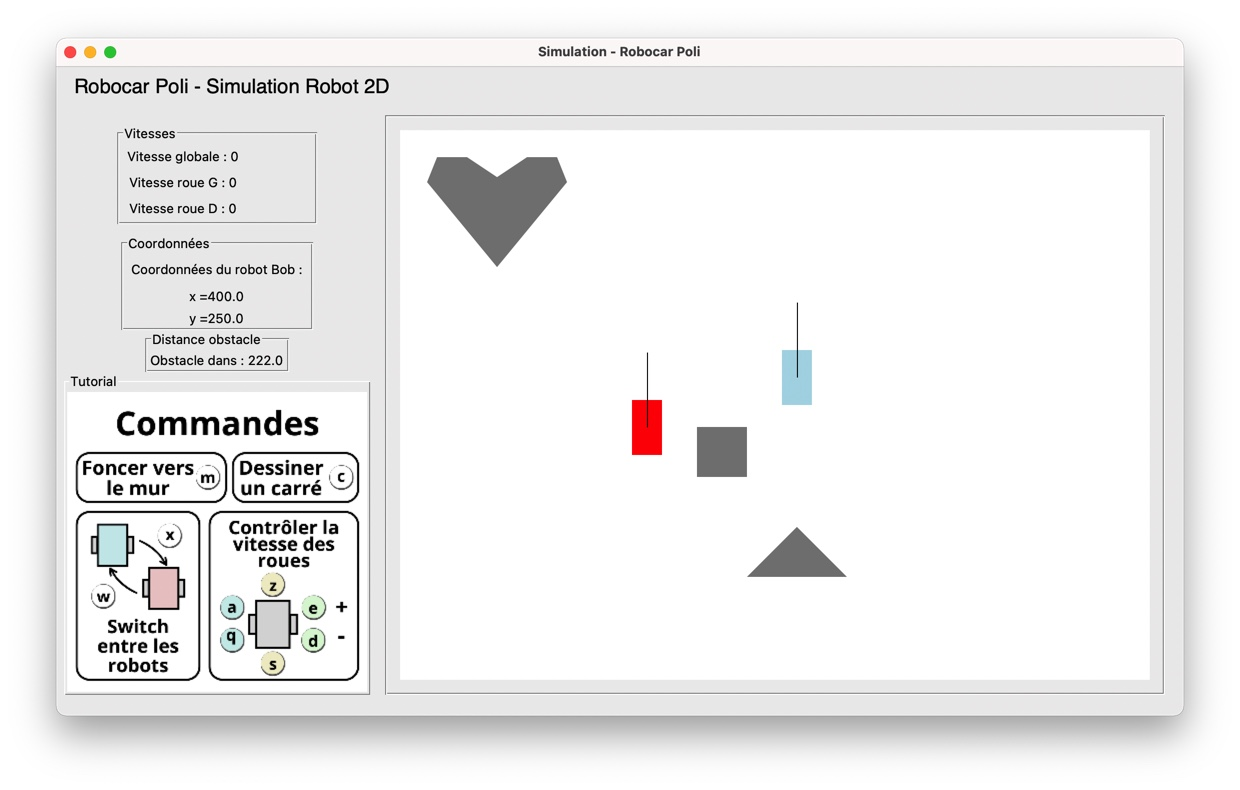
\includegraphics[width=1\linewidth]{image5.jpg} 
  \caption{Interface 2D de démonstration}
  \label{fig:exemple} 
\end{figure}

\begin{figure}[p] 
  \centering 
  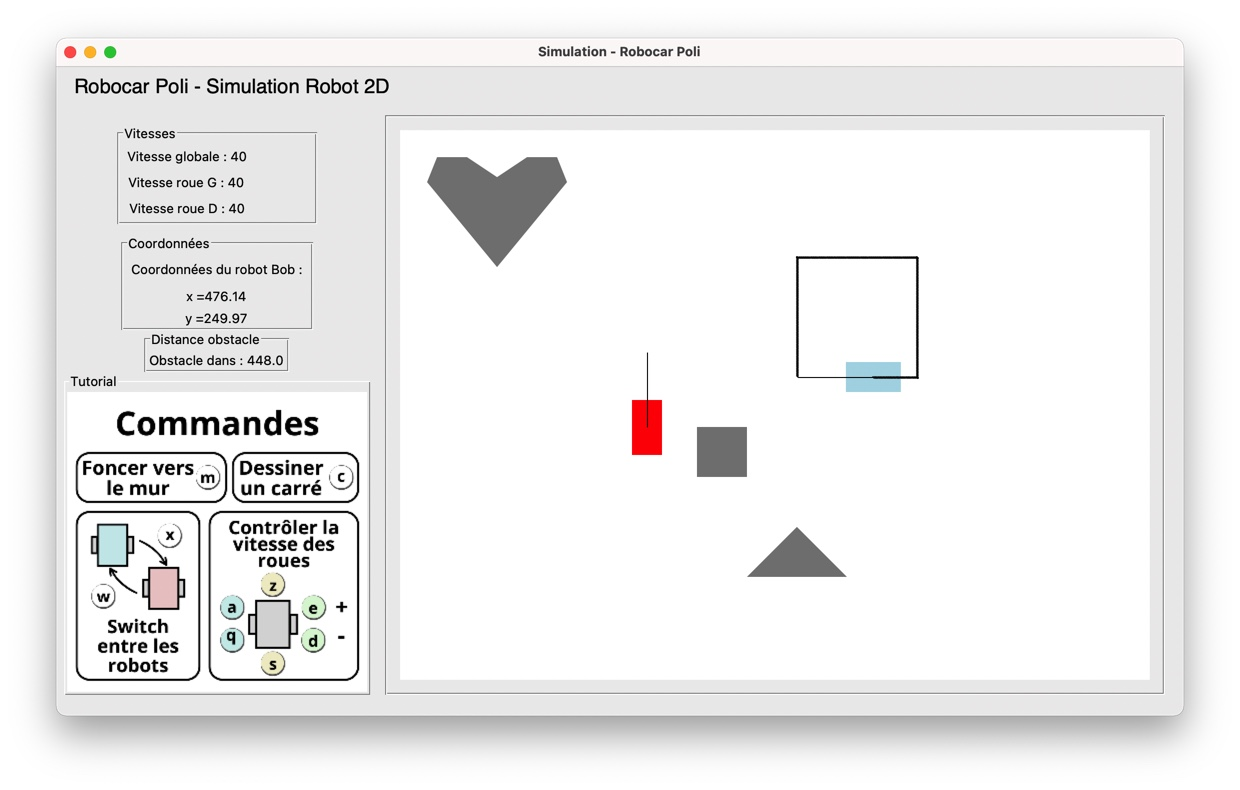
\includegraphics[width=1\linewidth]{image6.jpg} 
  \caption{Robot effectuant la stratégie “Tracer carré”}  
  \label{fig:exemple} 
\end{figure}

\begin{figure}[p]
  \centering 
  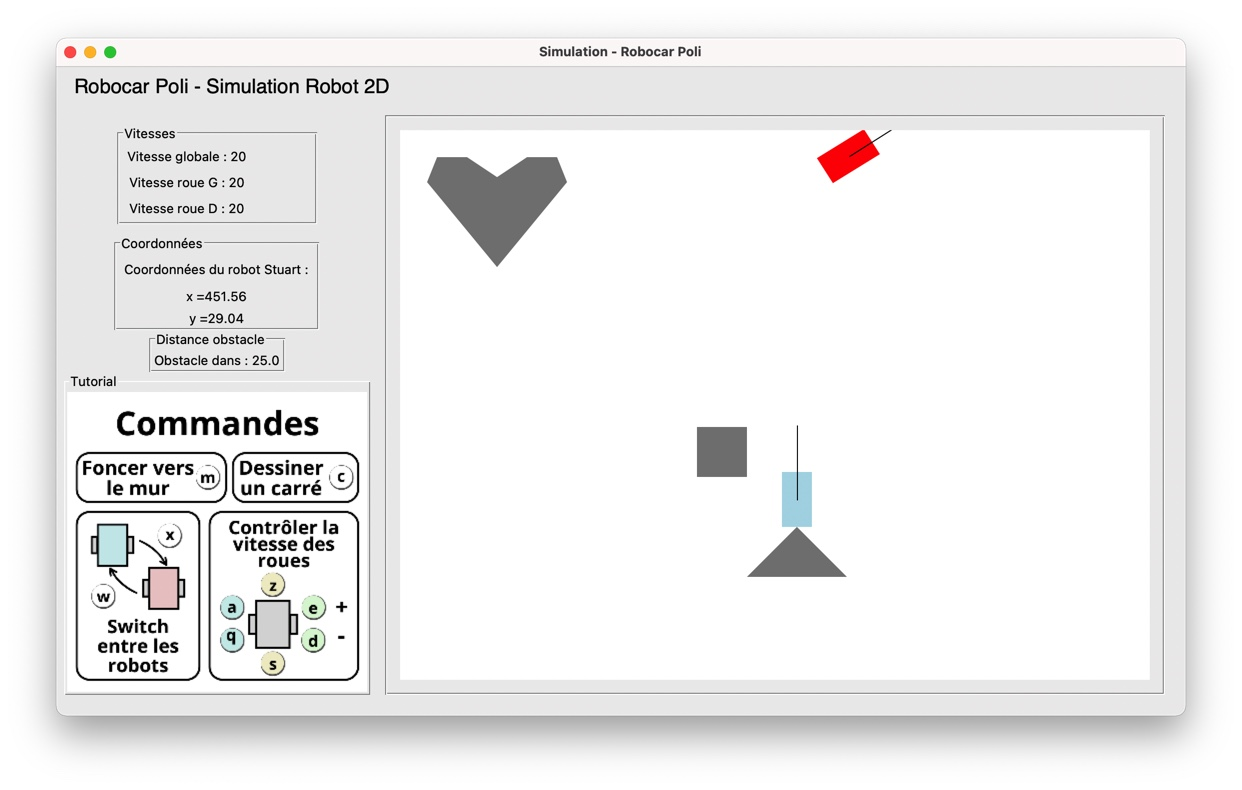
\includegraphics[width=1\linewidth]{image1.jpg} 
  \caption[Les deux robots crashés, Robot bleu dans un obstacle, robot rouge dans la bordure de l’interface]{\begin{varwidth}[t]{\linewidth}Les deux robots crashés, \\ Robot bleu dans un obstacle, robot rouge dans la bordure de l’interface\end{varwidth}}
  \label{fig:exemple} 
\end{figure}

\FloatBarrier

\end{center} 

\clearpage
\\
\subsection*{- Interface 3D et Robot réel} 
\addcontentsline{toc}{subsection}{Interface 3D et Robot réel}

\hspace{\parindent}Une fois notre interface 2D fonctionnelle et les stratégies correctement implémentées, nous avons pu avoir accès au \textbf{robot réel} (\texttt{Gopigo}). Nous avons alors mis en place les modules nécessaires pour faire le lien entre les stratégies développées et le Gopigo. Le robot pouvait alors effectuer les \textbf{stratégies} et le \textbf{déplacement libre}, comme dans notre interface 2D.

\hspace{\parindent}L'étape suivante de notre projet était alors d’implémenter la \textbf{stratégie de suivi de la balise}. 


\hspace{\parindent}Pour ce faire, nous avons dû créer une interface 3D. Notre choix s'est porté sur le module \textbf{Panda 3D} pour la réaliser. C’est un module \textbf{performant}, utilisé par plusieurs entreprises pour créer des jeux vidéos. Il permet de simuler un monde en 3D, d’y \textbf{inclure des objets} et de gérer des vues caméra. Il possède une documentation riche. Nous y avons facilement ajouté les éléments déjà présents dans l'interface 2D et ainsi que plusieurs vues : \textbf{vue du dessus} (\texttt{2D}), \textbf{vue arrière} et \textbf{vue avant} (simule la \texttt{caméra du robot}).

\hspace{\parindent}Par la suite, nous avons modélisé et ajouté une \textbf{balise} pour pouvoir simuler la stratégie de \textbf{suivi de balise}.

\begin{center}
\begin{figure}[h]
    \centering
    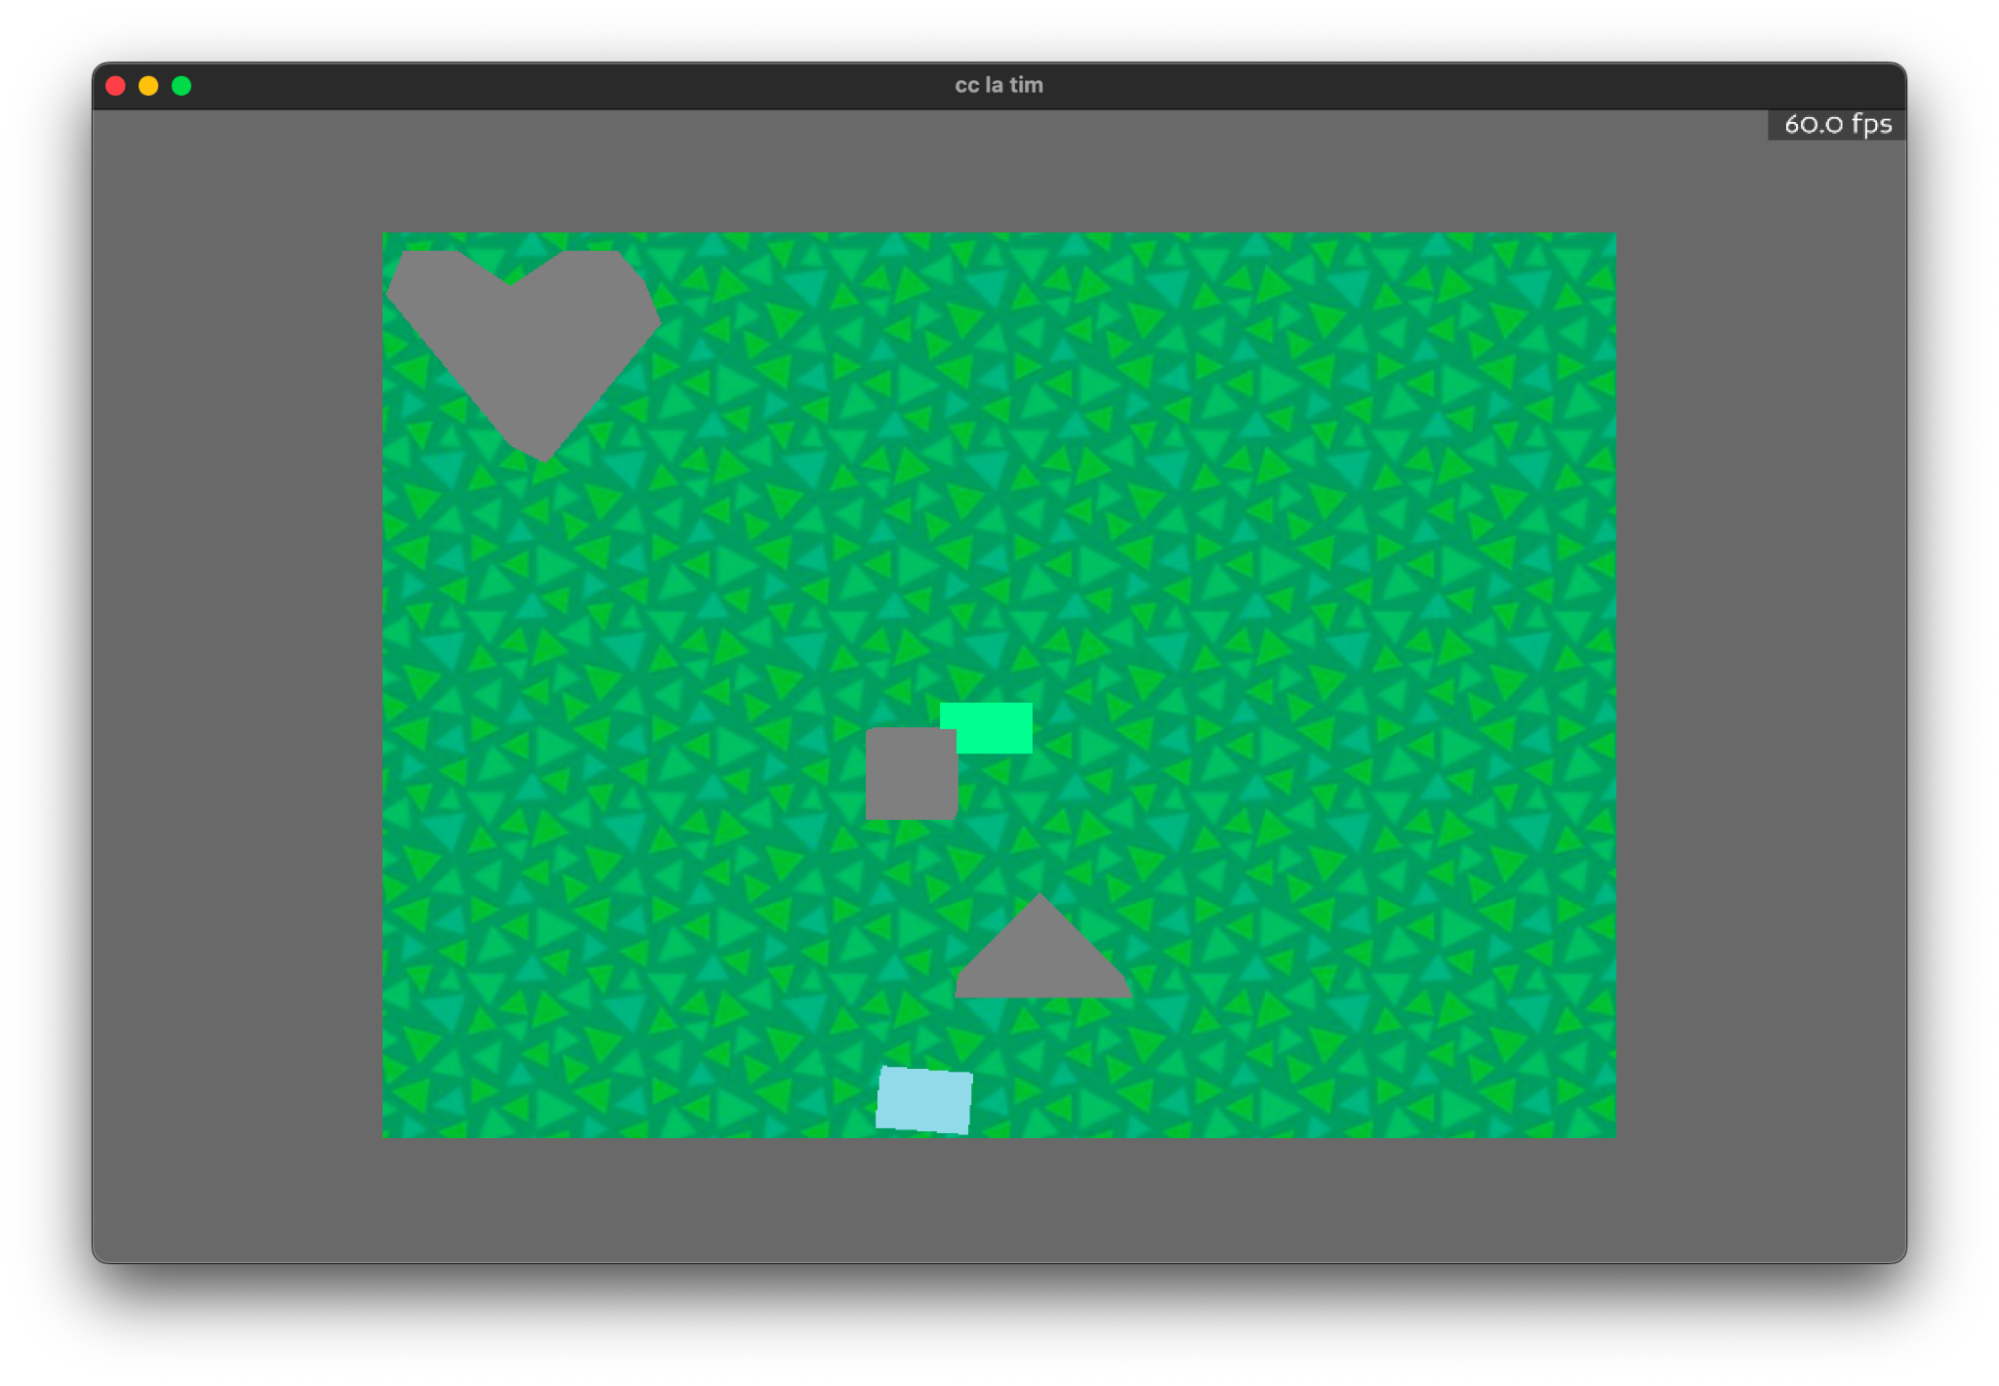
\includegraphics[width=1\linewidth]{image7.png}
    \caption{Vue du haut de l’interface 3D, avec les deux robots crash}
    \label{fig:enter-label}
\end{figure}



\begin{figure}[p]
    \centering
    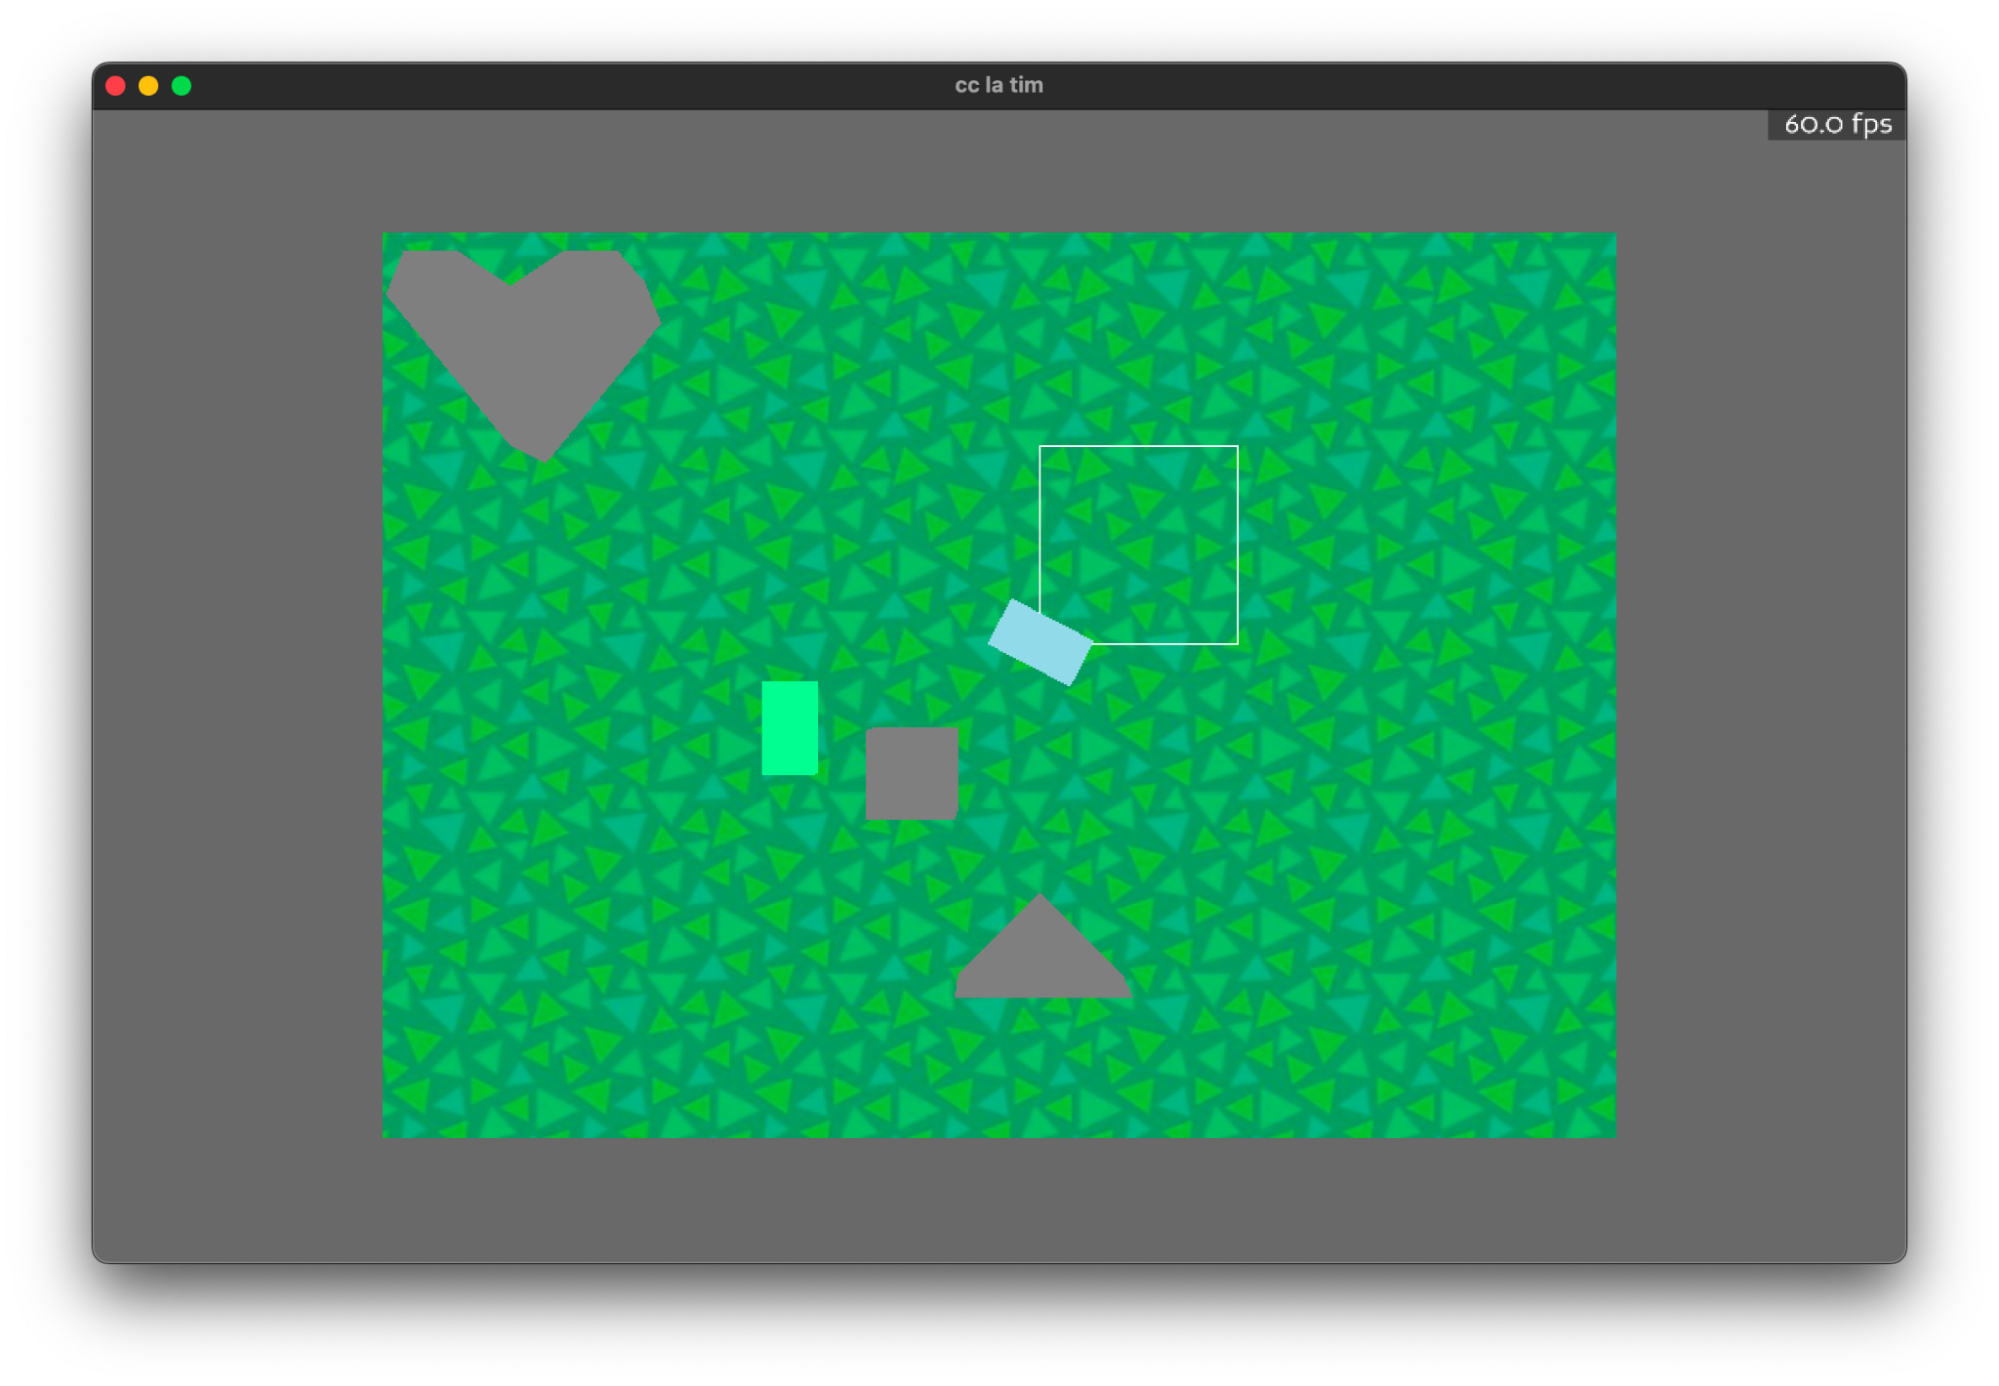
\includegraphics[width=1\linewidth]{image4.png}
    \caption{Vue de haut de l’interface 3D, avec "tracer carré" effectué}
    \label{fig:enter-label}
\end{figure}


\begin{figure}[p]
  \centering 
  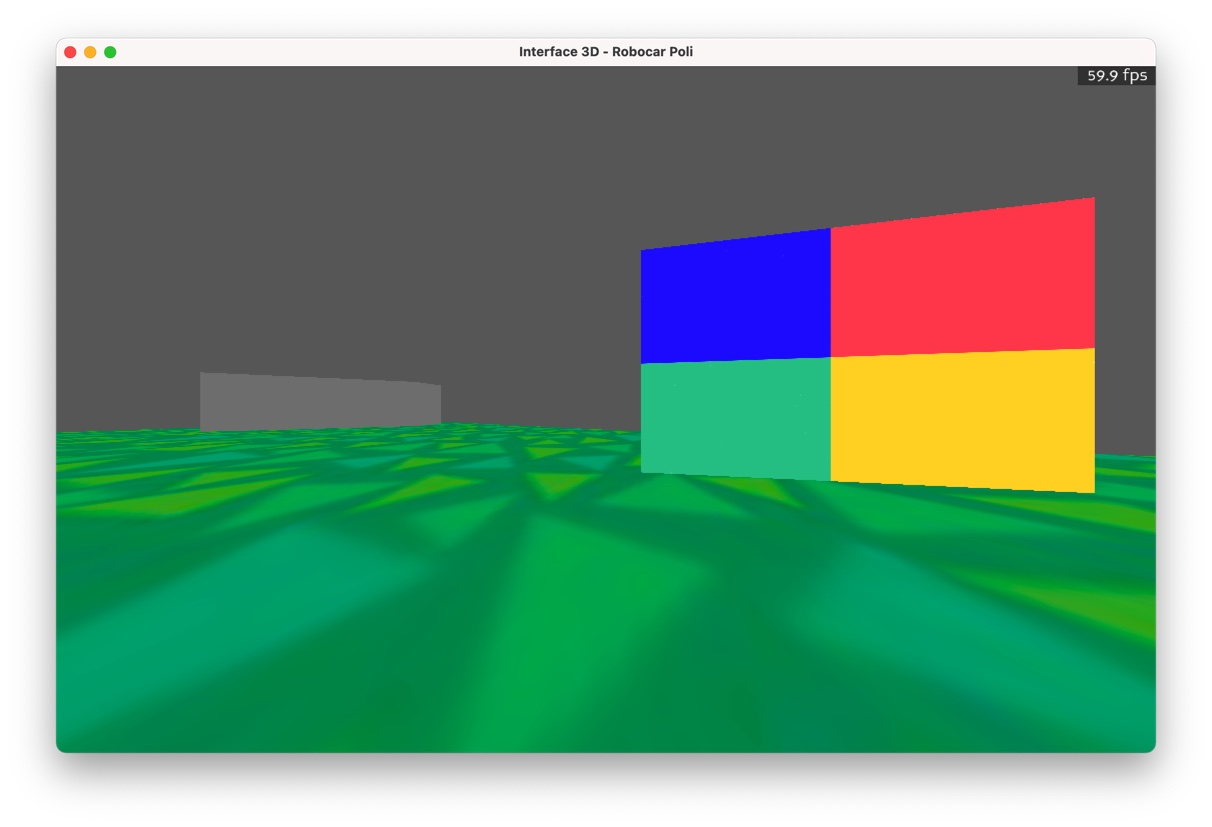
\includegraphics[width=1\linewidth]{image2.jpg} 
  \caption{Vue de devant, avec la balise devant le robot} 
  \label{fig:exemple}
\end{figure}

\begin{figure}[h]
    \centering
    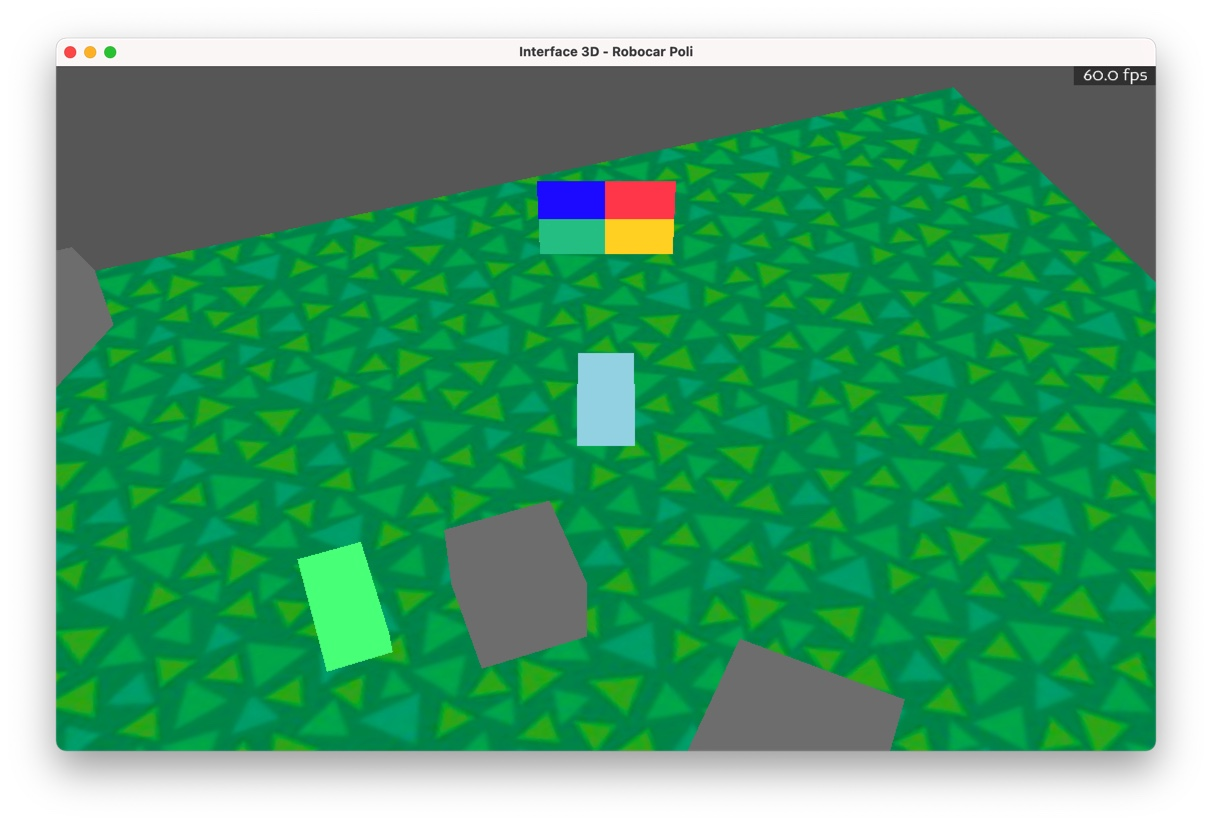
\includegraphics[width=1\linewidth]{image3.jpg}
    \caption{Vue arrière, avec la balise devant le robot}
    \label{fig:enter-label}
\end{figure}
\end{center} 

\FloatBarrier

\hspace{\parindent}En parallèle, nous testions nos stratégies sur le robot réel. Plusieurs \textbf{changements} ont alors dû être faits, par rapport à notre vision du robot simulé. Nous avons par exemple dû modifier notre manière de calculer les \textbf{rotations} des roues ou encore gérer les fonctionnalités propres au robot Gopigo comme les \textbf{offset des roues}. 

\hspace{\parindent}Nous nous sommes aussi intéressés à l'utilisation de la caméra du robot ainsi qu'à la \textbf{reconnaissance d'une balise}. La première étape était d'essayer de prendre plusieurs photos avec le robot, non sans difficulté. Il a ensuite fallu mettre au point une méthode de reconnaissance de la balise à l'aide du module \textbf{CV2}. Il s'agit d'une version adaptée de la bibliothèque \textbf{OpenCV}, utilisée pour du traitement d'images. Nous avons utilisé des \textbf{masks} pour détecter les quatre couleurs composant la balise. Ces derniers permettent d'obtenir des points (coordonnées) moyens pour chaque couleur trouvée, à partir desquels on peut déduire un point représentant le centre de la balise. Grâce à cette méthode, nous avons pu implémenter une nouvelle stratégie pour \textbf{reconnaître et suivre} la balise.


%--------------------------------------------------------------------
\\
\clearpage
\\
\section*{Architecture globale de notre projet}
\addcontentsline{toc}{section}{Architecture globale de notre projet} 

\subsection*{- Description générale}
\addcontentsline{toc}{subsection}{Description générale} 

% J'AI FAIS CA POUR L ARCHI MAIS CHANGER OU SUPP TOUS SI CA CONVIENT PAS :) -maelle
Le projet se trouve dans le répertoire Projet-2IN013. Il est structuré en trois dossiers et quatre fichiers exécutables, en plus des fichiers de test unitaires : 
\begin{itemize}[label=-]
    \item \texttt{autre} comporte les fiches, les comptes-rendus de chaque séance, les différentes photos prises et un diagramme UML du projet.
    \item \texttt{src} est un module dans lequel se trouvent quatre fichiers \texttt{constantes.py}, \texttt{environn-\\ement.py}, \texttt{obstacle.py} et \texttt{outils.py}. Les fichiers \texttt{constantes.py} et \texttt{outils.py} nous permettent de définir des valeurs numériques et des fonctions utiles utilisées à travers le projet. \texttt{obstacle.py} contient la classe \texttt{Obstacle} nous permettant de définir les obstacles utilisés dans nos simulations, alors que \texttt{environnement.py} contient la définition de l'environnement simulé, ainsi que toutes les méthodes qui permettent de le manipuler.
    
    De plus, \texttt{src} contient quatre sous modules. Tout d'abord, \texttt{interface2D} et \texttt{interf-\\ace3D} définissent les simulations d'interface en 2D et 3D respectivement, ainsi qu'une \texttt{démo} qui permet de créer un exemple d'interface générique qui peut être utilisé par l'utilisateur ou d'autres programmes du projet. On trouve dans le sous-module \texttt{controleur} tout ce qui est relatif à la gestion du contrôleur (qui agit sur le robot en lui donnant des instructions) ainsi qu'à la création des stratégies. Pour finir, le sous-module \texttt{robots} permet la définition de notre objet central, le robot (simulé avec \texttt{robot.py}, mockup du réel avec \texttt{mockupRobot.py} et réel avec \texttt{gopigo.py}), ainsi que des adaptateurs de chacun des robots. Les adaptateurs ont le rôle d'interprète entre le contrôleur et des robots de chaque type, en transmettant les ordres du contrôleur. \texttt{adapt.py} est la classe abstraite des Adaptateurs, dont héritent les adaptateurs des robots.
    
    \item \texttt{Test} contient les tests unitaires de chaque fonction du projet pouvant nécessiter un test.
    \item \texttt{main2D.py} permet de démarrer l'interface2D.
    \item \texttt{main3D.py} permet de lancer l'interface3D.
    \item \texttt{mainALL.py} permet d'exécuter les deux interfaces (une à la fois) sans fermer le programme. (la position des robots reste la même d'une interface à l'autre)
    \item \texttt{mainIRL.py} permet au robot réel de faire les différentes stratégies du contrôleur.
\end{itemize}
\\
Il est nécessaire de noter que, dans chaque module ou sous-module, il y a un fichier \texttt{\_\_init\_\_.py} qui facilite les import en récupérant les méthodes, constantes ou instances qui pourraient être nécessaires en dehors du module.

\subsection*{- Diagramme UML}
\addcontentsline{toc}{subsection}{Diagramme UML} 
\hspace{\parindent}Notre projet dans son ensemble peut être représenté par le diagramme UML suivant. Le diagramme nous permet de voir les méthodes et attributs présents dans chaque module ainsi que les liens entre les modules. \\

\begin{landscape}
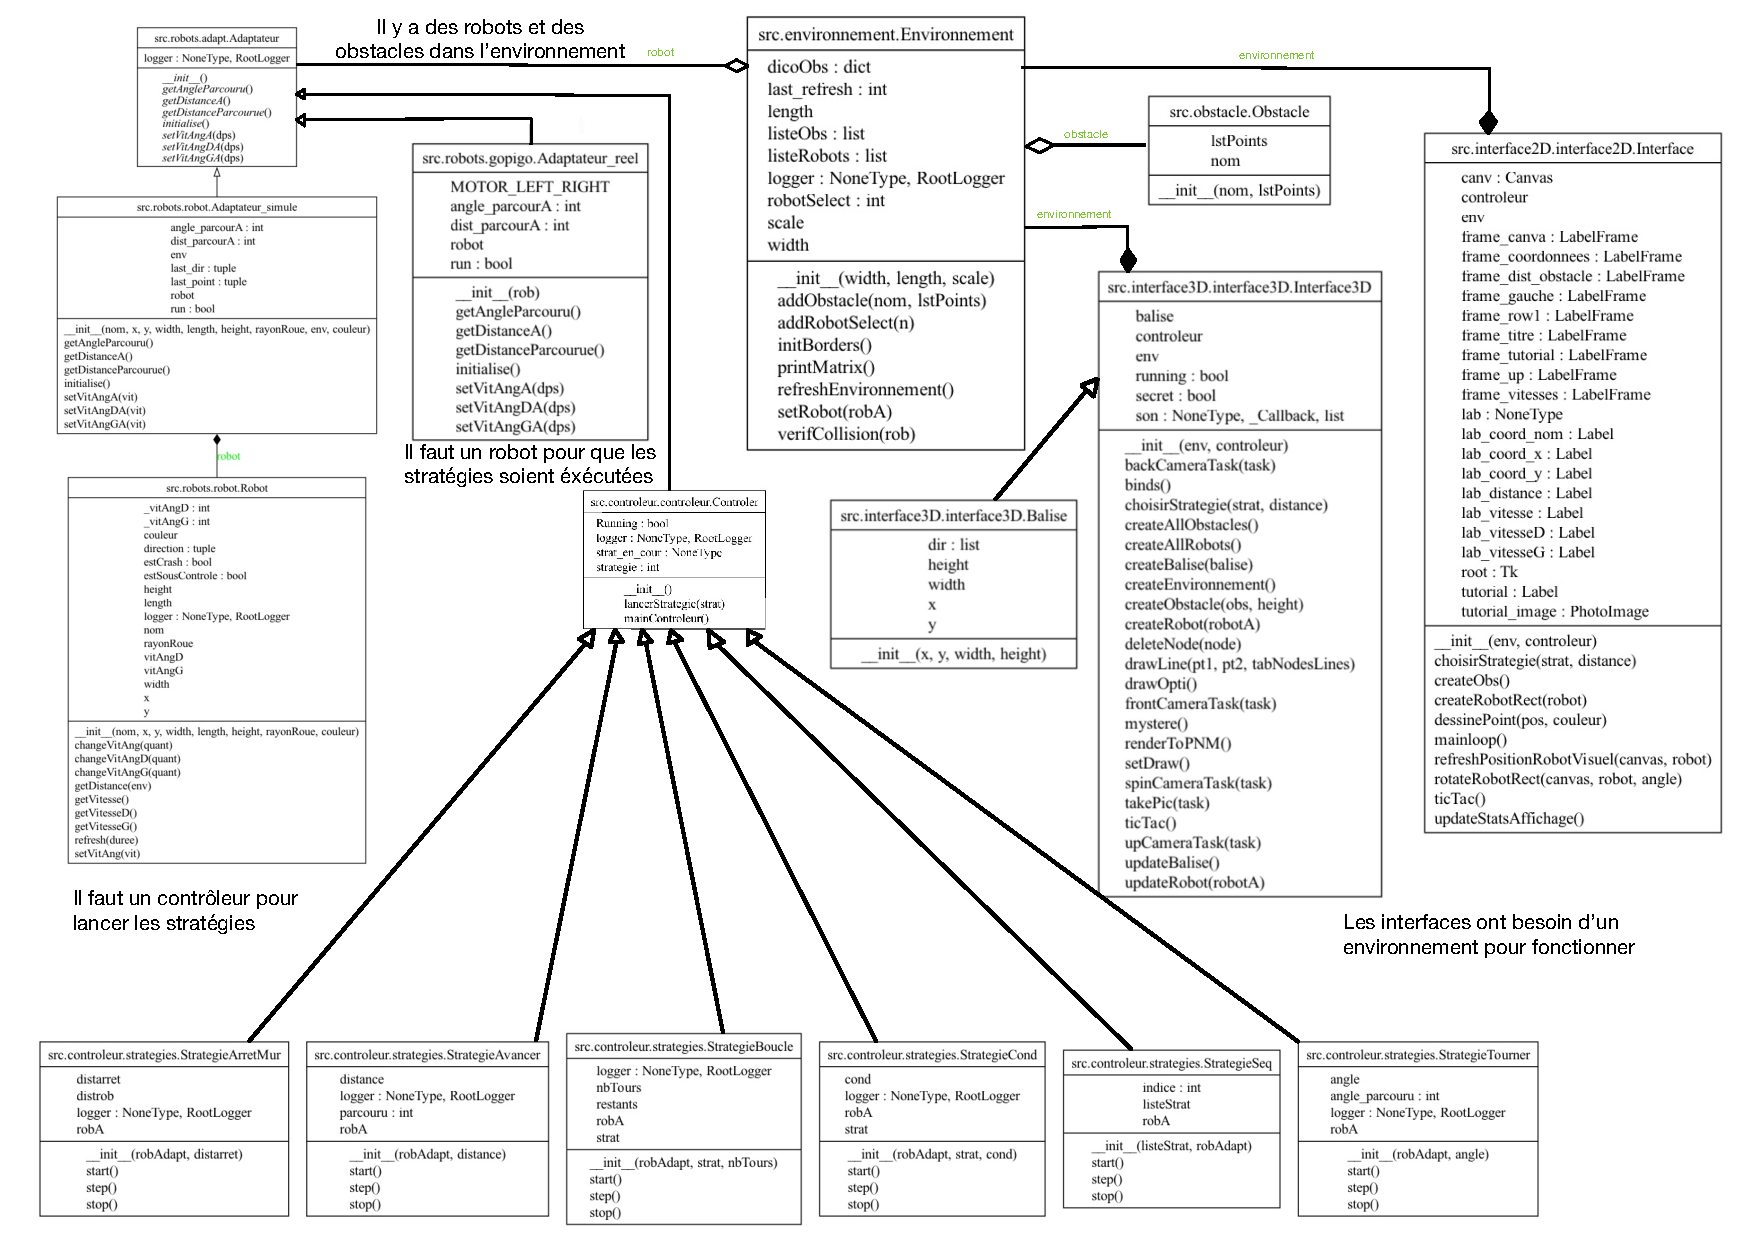
\includepdf[pages=1,angle=90, fitpaper=true]{UML2.pdf}
\end{landscape}
 % \includepdf[pages=1,fitpaper=true]{path/to/yourfile.pdf}
\\

\clearpage
\section*{Gestion du travail en groupe}
\addcontentsline{toc}{section}{Gestion du travail en groupe}

\hspace{\parindent}Pour la gestion de notre projet, nous avons utilisé deux outils principaux : \textbf{Github} pour la partie code et \textbf{Trello }pour la partie organisationnelle. Ils nous ont permis, sur toute la durée du projet, d’avoir une prise en main accompagnée et facilitée.

\hspace{\parindent}La méthode\textbf{ Agile}, avec les \textbf{Scrums} à compléter chaque semaine, a donné une certaine consistance dans notre projet, afin de répondre aux exigences de nos \textbf{clients} et de leur présenter une démonstration chaque semaine. La fragmentation des objectifs en tâches unitaires nous a offert une meilleure prise en main et répartition du travail, et nous arrivions en général assez bien à nous approprier les différentes tâches. La répartition des tâches se faisait ensuite de manière assez naturelle.

\hspace{\parindent} Github a été très utile d’un point de vue pratique pour nous permettre de travailler à plusieurs sur le projet, mais également sur plusieurs éléments différents en parallèle grâce aux \textbf{branches}. Nous pouvions ainsi développer différentes parties du projet \textbf{séparément} sans dépendre de l’avancée du travail d’une autre personne.

\hspace{\parindent}Nous organisions des \textbf{réunions hebdomadaires} en milieu de Sprint afin de faire un point sur l’avancée des tâches, mais surtout afin de partager d’éventuels problèmes rencontrés et de réfléchir à des solutions. En plus de ces réunions, nous avions également des séances de \textbf{brainstorming} avec tous ou bien une partie des membres du groupe selon la complexité de la fonctionnalité dont il était question.
 


\section*{Perspectives d'amélioration}
\addcontentsline{toc}{section}{Perspectives d'amélioration}

\hspace{\parindent}Avec le recul, il y a quelques points sur lesquels nous aurions pu nous améliorer pour ce projet. En effet, nous n’avons pas utilisé toutes les fonctionnalités dont le robot dispose. C'est dommage car il y a de nombreuses options qui auraient permis de réaliser des stratégies \textbf{innovantes} et \textbf{intéressantes}, comme l'utilisation du \textbf{servo} (tête rotative).

\hspace{\parindent}Un autre aspect sur lequel nous aurions pu être plus performants est la \textbf{consistance} et la répartition du travail. Vers la fin du projet, le travail était plus déséquilibré entre les membres de l’équipe. Nous étions moins réguliers et nous aurions pu avoir une meilleure distribution des tâches entre co-équipiers (les examens des autres UE ont également eu un impact sur la quantité de travail fournie sur le projet).

\hspace{\parindent} Enfin, nous n'avons pas trouvé de moyen assez rapide et efficace pour \textbf{récupérer une image} de la vue avant du robot dans Panda3D. Sans ce problème, notre stratégie aurait été beaucoup plus performante dans la simulation. Il est à noter que cette stratégie fonctionne \textbf{parfaitement} sur le robot réel. 


\newpage
\section*{Conclusion}
\addcontentsline{toc}{section}{Conclusion}

\subsection*{- Ce qui nous distingue des autres}
\addcontentsline{toc}{subsection}{Ce qui nous distingue des autres}

\hspace{\parindent}De nombreux points de notre projet le rendent \textbf{original} et le distinguent des autres, tant au niveau de l’implémentation que de l’utilisation. 

\hspace{\parindent}Tout d’abord, en ce qui concerne la partie simulée, nous utilisons les \textbf{threads}, ce qui nous permet d’avoir des robots qui fonctionnent \textbf{indépendamment} des simulations. Ils continuent donc à être en activité même si on \textbf{ferme une interface} (pour arrêter le robot il faut arrêter le programme). Notre interface 3D nous permet d’avoir \textbf{3} points de vue différents, un point de vue omniscient (équivalent au point de vue de la simulation 2D), un point de vue de l'arrière du robot, et un point de vue première personne, simulant la caméra à l'avant du robot réel. 

\begin{figure}[h]
    \centering
    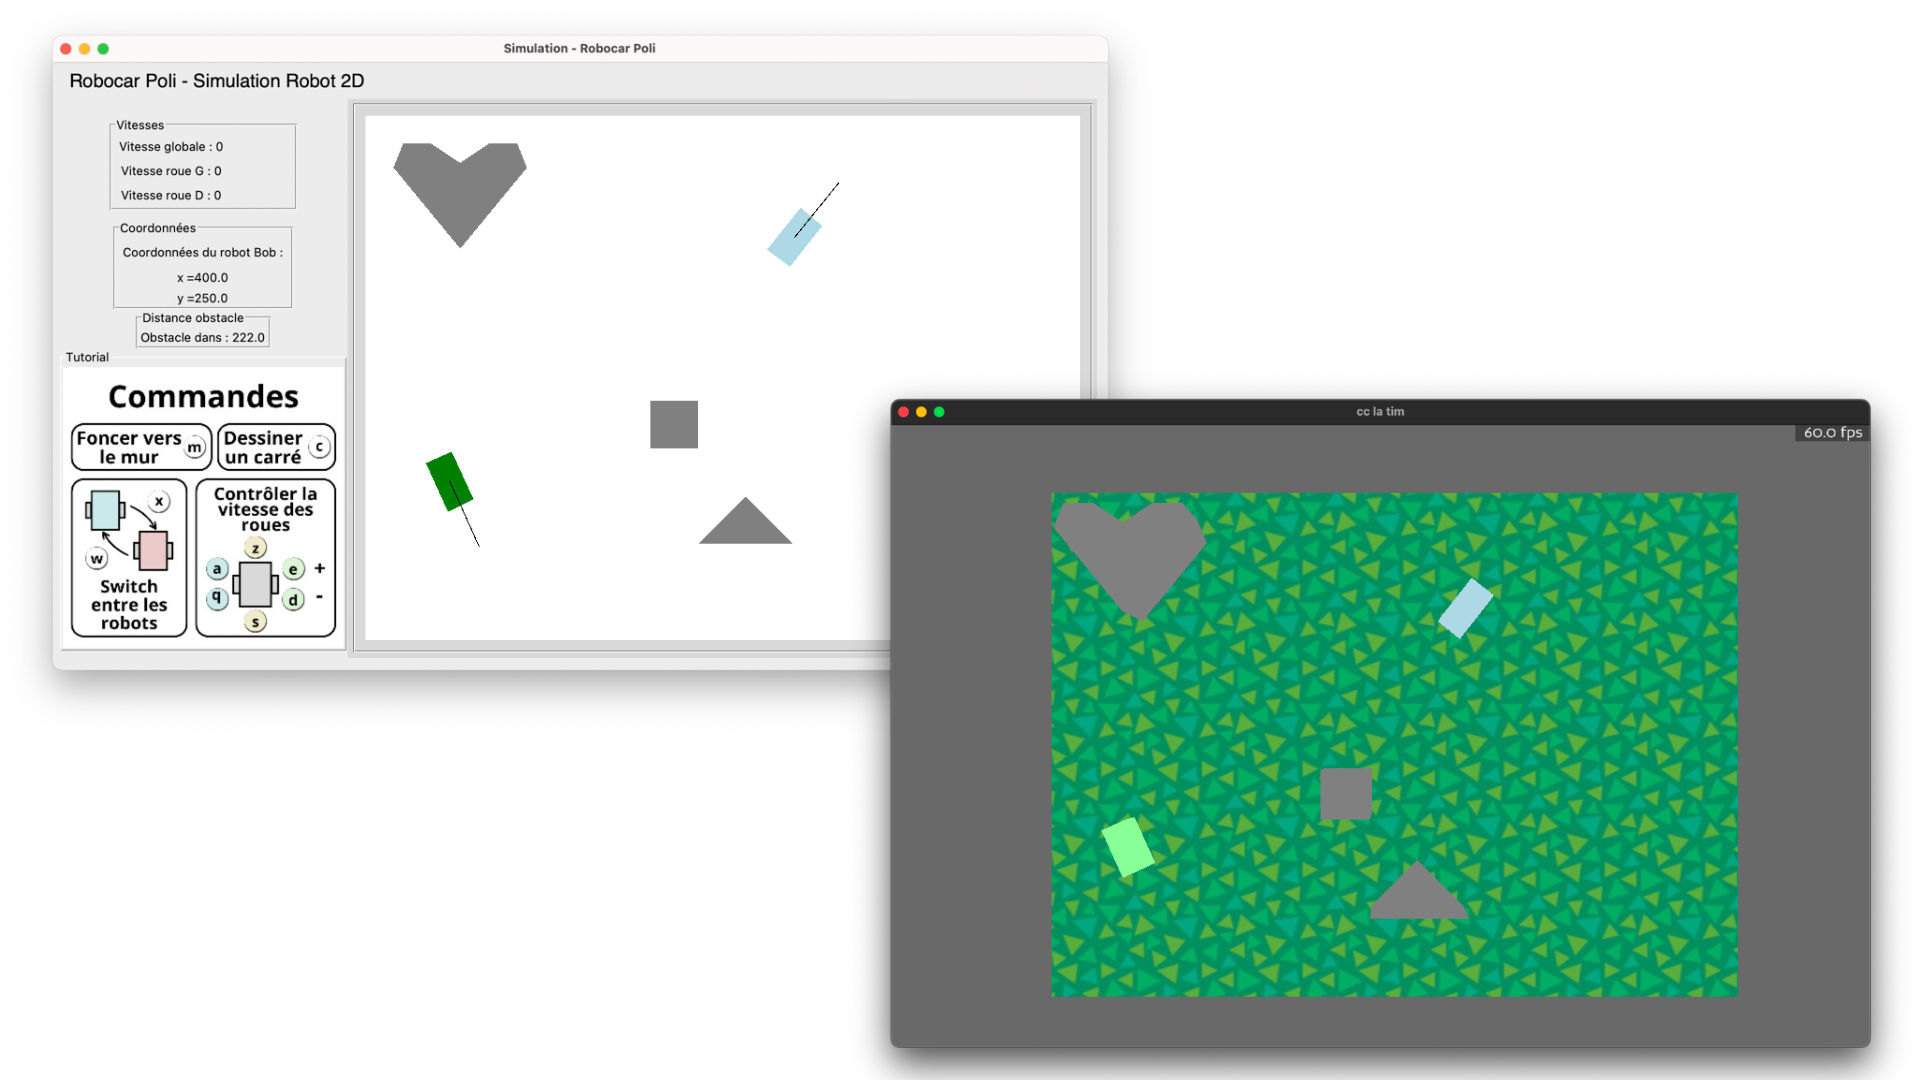
\includegraphics[width=1\linewidth]{double.png}
    \caption{Interfaces 2D et 3D ouvertes pour le même environnement}
    \label{fig:enter-label}
\end{figure}

\hspace{\parindent}Nous pouvons également ajouter des obstacles de forme \textbf{personnalisée} dans les simulations. Cela donne au client une représentation plus fidèle de la réalité et plus de flexibilité. De plus, il est possible de contrôler les mouvements du robot en dehors des stratégies définies, en modulant les vitesses des roues individuellement avec les touches du clavier.

\hspace{\parindent}D’un point de vue plus pratique, nous avons également résolu des problèmes avec le robot. Nous avons \textbf{remonté} le robot lorsqu’il était cassé, et nous avons retourné la caméra d’un des robots qui se tenait \textbf{à l’envers}. De plus, nous avons remarqué de petites inconsistances de l’API qui posaient des problèmes lors de l’acquisition d’images, et qui pouvaient \textbf{bloquer d’autres tentatives} d’utilisation de la caméra et d’instanciation du robot. Une fois qu'un robot était instancié pour la première fois, la caméra n'était plus utilisable avec une instance différente. Cela nous forçait à redémarrer le robot à chaque fois.


\clearpage
\hspace{\parindent} Pour finir, une autre caractéristique qui nous démarque est la stratégie supplémentaire que nous avons conçue. En effet, elle montre notre compréhension des axes du projet et nous permet d'aller au-delà de ses objectifs, en utilisant différentes fonctionnalités à la fois : mouvement, son et lumière, le tout en respectant le thème Robocar Poli de notre groupe : la boucle est bouclée ! \\


\subsection*{- Avis sur le projet}
\addcontentsline{toc}{subsection}{Avis sur le projet}

\hspace{\parindent}En rétrospective, ce projet a pu être très frustrant par  moments, mais il nous a apporté de l’\textbf{expérience} et des \textbf{compétences} précieuses. 

\hspace{\parindent}Il nous a appris à travailler en équipe sur notre premier projet de grande ampleur, en terme de temps, d'objectifs, ou de travail fourni. Nous avons été introduits aux méthodes de travail Agile et Scrum. Ces méthodes étaient pour nous une première, qui présentent l'avantage d'une meilleure gestion de projet lorsque le nombre de tâches est important. Elles sont aussi très utiles quand le projet comporte plusieurs membres dans l’équipe, comme ici. Ces outils nous ont guidés dans notre manière de nous organiser et nous ont permis de maintenir un rythme de travail \textbf{stable}, semaine après semaine, afin de répondre aux attentes de nos \textbf{professeurs}. 

\hspace{\parindent}Nous avons aussi été confrontés à la gestion de problèmes en tous genres. Nous avons dû chercher des \textbf{solutions} à ces problèmes en trouvant des personnes qui ont fait face à des situations similaires (sur des forums, par exemple), à nos \textbf{membres de groupe}, voire à d’autres \textbf{camarades} de classe.

\hspace{\parindent}Le projet était intéressant dans la mesure où nous avons pu voir une \textbf{application concrète} de notre travail avec un robot \textbf{physique} qui répondait à nos commandes. Cela le distingue des autres travaux que nous avons pu faire jusqu’alors dans d'autres UE. Leur influence était limitée à nos ordinateurs. Nous avons pu nous \textbf{amuser} à voir nos programmes avoir une incidence sur le monde physique. De plus, voir notre projet \textbf{se construire} et avancer chaque semaine a été satisfaisant pour nous. Savoir que nous partions d'un dossier vide nous rend d'autant plus \textbf{fiers}.

\\

\clearpage
\section*{Remerciements}
\addcontentsline{toc}{section}{Remerciements}
\\

Enfin, nous souhaitons remercier nos deux professeurs \textbf{M. Baskiotis} et \textbf{M. Sigaud}.\textbf{} \\

\hspace{\parindent}\textbf{Merci} pour vos conseils précieux chaque semaine. Les rendez-vous avec vous ont au départ été exigeants et parfois "démoralisants", mais vous avez tous les deux su nous donner de la rigueur, de la \textbf{motivation} et une vision claire de notre projet. Grâce à votre encadrement et votre \textbf{soutien}, nous avons pu surmonter les obstacles et \textbf{progresser} de manière significative. Votre expertise et votre patience ont été \textbf{inestimables}, et nous vous en sommes \textbf{profondément reconnaissants}. 
% svp on peut rajouter ca ? (emoji avec les gros yeux)
\\
Nous espérons avoir su vous montrer nos compétences et vous convaincre, en tant que client, de choisir notre entreprise pour la réalisation de votre projet !

\\
\end{document}
